% Options for packages loaded elsewhere
\PassOptionsToPackage{unicode}{hyperref}
\PassOptionsToPackage{hyphens}{url}
%
\documentclass[
]{article}
\title{Outbreak response models of vaccine-preventable diseases in
humans (1970-2019) - A systematic review (Primary Analysis)}
\author{James Azam}
\date{November 05, 2021}

\usepackage{amsmath,amssymb}
\usepackage{lmodern}
\usepackage{iftex}
\ifPDFTeX
  \usepackage[T1]{fontenc}
  \usepackage[utf8]{inputenc}
  \usepackage{textcomp} % provide euro and other symbols
\else % if luatex or xetex
  \usepackage{unicode-math}
  \defaultfontfeatures{Scale=MatchLowercase}
  \defaultfontfeatures[\rmfamily]{Ligatures=TeX,Scale=1}
\fi
% Use upquote if available, for straight quotes in verbatim environments
\IfFileExists{upquote.sty}{\usepackage{upquote}}{}
\IfFileExists{microtype.sty}{% use microtype if available
  \usepackage[]{microtype}
  \UseMicrotypeSet[protrusion]{basicmath} % disable protrusion for tt fonts
}{}
\makeatletter
\@ifundefined{KOMAClassName}{% if non-KOMA class
  \IfFileExists{parskip.sty}{%
    \usepackage{parskip}
  }{% else
    \setlength{\parindent}{0pt}
    \setlength{\parskip}{6pt plus 2pt minus 1pt}}
}{% if KOMA class
  \KOMAoptions{parskip=half}}
\makeatother
\usepackage{xcolor}
\IfFileExists{xurl.sty}{\usepackage{xurl}}{} % add URL line breaks if available
\IfFileExists{bookmark.sty}{\usepackage{bookmark}}{\usepackage{hyperref}}
\hypersetup{
  pdftitle={Outbreak response models of vaccine-preventable diseases in humans (1970-2019) - A systematic review (Primary Analysis)},
  pdfauthor={James Azam},
  hidelinks,
  pdfcreator={LaTeX via pandoc}}
\urlstyle{same} % disable monospaced font for URLs
\usepackage[margin=1in]{geometry}
\usepackage{longtable,booktabs,array}
\usepackage{calc} % for calculating minipage widths
% Correct order of tables after \paragraph or \subparagraph
\usepackage{etoolbox}
\makeatletter
\patchcmd\longtable{\par}{\if@noskipsec\mbox{}\fi\par}{}{}
\makeatother
% Allow footnotes in longtable head/foot
\IfFileExists{footnotehyper.sty}{\usepackage{footnotehyper}}{\usepackage{footnote}}
\makesavenoteenv{longtable}
\usepackage{graphicx}
\makeatletter
\def\maxwidth{\ifdim\Gin@nat@width>\linewidth\linewidth\else\Gin@nat@width\fi}
\def\maxheight{\ifdim\Gin@nat@height>\textheight\textheight\else\Gin@nat@height\fi}
\makeatother
% Scale images if necessary, so that they will not overflow the page
% margins by default, and it is still possible to overwrite the defaults
% using explicit options in \includegraphics[width, height, ...]{}
\setkeys{Gin}{width=\maxwidth,height=\maxheight,keepaspectratio}
% Set default figure placement to htbp
\makeatletter
\def\fps@figure{htbp}
\makeatother
\setlength{\emergencystretch}{3em} % prevent overfull lines
\providecommand{\tightlist}{%
  \setlength{\itemsep}{0pt}\setlength{\parskip}{0pt}}
\setcounter{secnumdepth}{-\maxdimen} % remove section numbering
\ifLuaTeX
  \usepackage{selnolig}  % disable illegal ligatures
\fi

\begin{document}
\maketitle

{
\setcounter{tocdepth}{2}
\tableofcontents
}
We did not include foot and mouth disease (FMD) in all the primary
analyses. All analyses pertaining to FMD can be found in the
supplementary files.

\hypertarget{publications-per-year}{%
\section{Publications per year}\label{publications-per-year}}

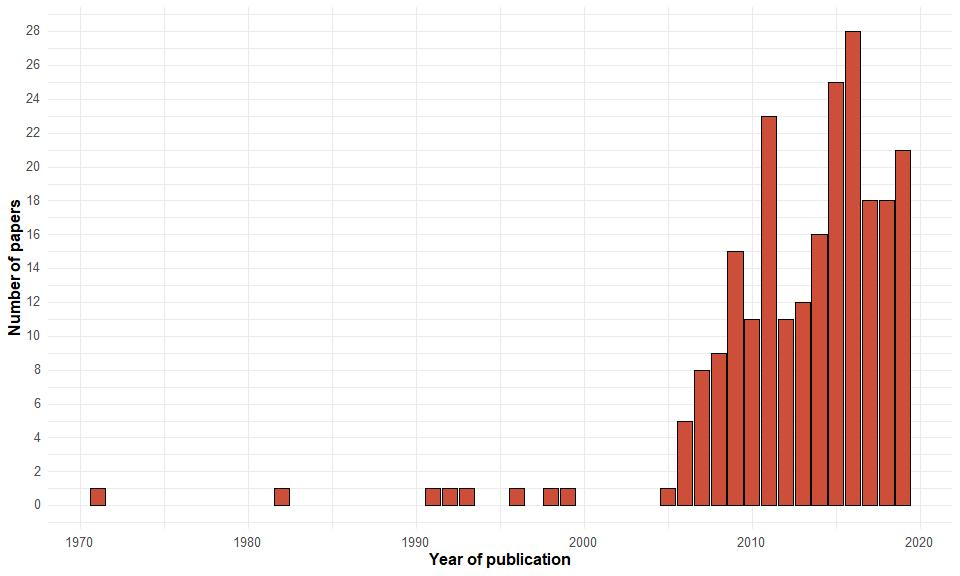
\includegraphics{orv_sys_rev_data_analysis_files/figure-latex/unnamed-chunk-3-1.jpeg}

\hypertarget{primary-objectives-of-review}{%
\section{Primary objectives of
review}\label{primary-objectives-of-review}}

\hypertarget{collaboration-patterns-in-time}{%
\subsection{Collaboration patterns in
time}\label{collaboration-patterns-in-time}}

\hypertarget{number-of-studies-per-combinations-of-collaboration-types}{%
\subsubsection{Number of studies per combinations of collaboration
types}\label{number-of-studies-per-combinations-of-collaboration-types}}

\begin{longtable}[]{@{}ll@{}}
\toprule
author\_affiliation\_type & n \\
\midrule
\endhead
academic\_institutions & 57.2\% (131) \\
academic\_institutions + government\_institutions & 24.0\% (55) \\
academic\_institutions + NGO & 7.4\% (17) \\
academic\_institutions + government\_institutions + NGO & 6.1\% (14) \\
government\_institutions & 2.2\% (5) \\
NGO & 2.2\% (5) \\
government\_institutions + NGO & 0.9\% (2) \\
Total & 100.0\% (229) \\
\bottomrule
\end{longtable}

\hypertarget{proportions-of-the-total-publications-per-year-by-collaboration-type}{%
\subsubsection{Proportions of the total publications per year by
collaboration
type}\label{proportions-of-the-total-publications-per-year-by-collaboration-type}}

\includegraphics{orv_sys_rev_data_analysis_files/figure-latex/unnamed-chunk-5-1.jpeg}

\hypertarget{absolute-number-of-publications-per-year-by-collaboration-type}{%
\subsubsection{Absolute number of publications per year by collaboration
type}\label{absolute-number-of-publications-per-year-by-collaboration-type}}

\includegraphics{orv_sys_rev_data_analysis_files/figure-latex/unnamed-chunk-6-1.jpeg}

Even though non-academic collaborations increased over time, the share
of total publications per year over time decreased.

\hypertarget{collaboration-patterns-in-geographic-space}{%
\subsection{Collaboration patterns in geographic
space}\label{collaboration-patterns-in-geographic-space}}

\hypertarget{real-versus-hypothetical-locations}{%
\subsubsection{Real versus hypothetical
locations}\label{real-versus-hypothetical-locations}}

\begin{longtable}[]{@{}ll@{}}
\toprule
location\_type & n \\
\midrule
\endhead
real & 78.7\% (196) \\
none & 21.3\% (53) \\
Total & 100.0\% (249) \\
\bottomrule
\end{longtable}

\hypertarget{larger-than-one-country}{%
\subsubsection{Larger than one country}\label{larger-than-one-country}}

\begin{longtable}[]{@{}ll@{}}
\toprule
country\_studied & n \\
\midrule
\endhead
west\_africa & 47.4\% (9) \\
global & 36.8\% (7) \\
northern\_hemisphere & 5.3\% (1) \\
southeast\_asia & 5.3\% (1) \\
who\_southeast\_asia\_region & 5.3\% (1) \\
Total & 100.0\% (19) \\
\bottomrule
\end{longtable}

\hypertarget{countries-studied}{%
\subsubsection{Countries studied}\label{countries-studied}}

\begin{longtable}[]{@{}ll@{}}
\caption{Number of studies per country}\tabularnewline
\toprule
country\_studied & num\_of\_studies \\
\midrule
\endfirsthead
\toprule
country\_studied & num\_of\_studies \\
\midrule
\endhead
US & 21.5\% (38) \\
CN & 10.7\% (19) \\
CA & 6.2\% (11) \\
LR & 5.6\% (10) \\
HK & 5.1\% (9) \\
MX & 5.1\% (9) \\
\bottomrule
\end{longtable}

\hypertarget{continents-studied}{%
\subsubsection{Continents studied}\label{continents-studied}}

\begin{longtable}[]{@{}ll@{}}
\caption{Number of studies per continent}\tabularnewline
\toprule
continent\_studied & num\_of\_studies \\
\midrule
\endfirsthead
\toprule
continent\_studied & num\_of\_studies \\
\midrule
\endhead
americas & 36.2\% (68) \\
africa & 25.0\% (47) \\
asia & 25.0\% (47) \\
europe & 13.3\% (25) \\
oceania & 0.5\% (1) \\
Total & 100.0\% (188) \\
\bottomrule
\end{longtable}

\hypertarget{geographic-connection-of-authors-to-the-studied-locations}{%
\subsubsection{Geographic connection of authors to the studied
locations}\label{geographic-connection-of-authors-to-the-studied-locations}}

\hypertarget{top-5-countries}{%
\paragraph{Top 5 countries}\label{top-5-countries}}

\begin{longtable}[]{@{}llllr@{}}
\toprule
collab\_type & country\_studied & yes & no & Total \\
\midrule
\endhead
purely\_academic & US & 94.4\% (17) & 5.6\% (1) & 18 \\
purely\_academic & CN & 100.0\% (8) & 0.0\% (0) & 8 \\
purely\_academic & HK & 77.8\% (7) & 22.2\% (2) & 9 \\
purely\_academic & LR & 0.0\% (0) & 100.0\% (3) & 3 \\
purely\_academic & CA & 75.0\% (3) & 25.0\% (1) & 4 \\
mixed & US & 100.0\% (17) & 0.0\% (0) & 17 \\
mixed & CN & 100.0\% (11) & 0.0\% (0) & 11 \\
mixed & CA & 100.0\% (7) & 0.0\% (0) & 7 \\
mixed & MX & 80.0\% (4) & 20.0\% (1) & 5 \\
mixed & LR & 25.0\% (1) & 75.0\% (3) & 4 \\
Total & - & 87.2\% (75) & 12.8\% (11) & 86 \\
\bottomrule
\end{longtable}

\hypertarget{aggregated}{%
\paragraph{Aggregated}\label{aggregated}}

\begin{longtable}[]{@{}lllr@{}}
\toprule
collab\_type & yes & no & Total \\
\midrule
\endhead
mixed & 84.0\% (63) & 16.0\% (12) & 75 \\
purely\_academic & 66.3\% (55) & 33.7\% (28) & 83 \\
Total & 74.7\% (118) & 25.3\% (40) & 158 \\
\bottomrule
\end{longtable}

\hypertarget{diseases-studied-per-collab-type}{%
\subsection{Diseases studied per collab
type}\label{diseases-studied-per-collab-type}}

\begin{longtable}[]{@{}lllr@{}}
\caption{Number of studies per disease and collaboration
type}\tabularnewline
\toprule
disease & purely\_academic & mixed & Total \\
\midrule
\endfirsthead
\toprule
disease & purely\_academic & mixed & Total \\
\midrule
\endhead
Total & 56.5\% (134) & 43.5\% (103) & 237 \\
Influenza & 54.1\% (73) & 45.9\% (62) & 135 \\
Ebola & 71.4\% (25) & 28.6\% (10) & 35 \\
Dengue & 50.0\% (6) & 50.0\% (6) & 12 \\
Cholera & 81.8\% (9) & 18.2\% (2) & 11 \\
Measles & 36.4\% (4) & 63.6\% (7) & 11 \\
Tuberculosis & 85.7\% (6) & 14.3\% (1) & 7 \\
Poliomyelitis & 28.6\% (2) & 71.4\% (5) & 7 \\
Varicella & 50.0\% (2) & 50.0\% (2) & 4 \\
Meningococcal meningitis & 33.3\% (1) & 66.7\% (2) & 3 \\
Pertussis & 50.0\% (1) & 50.0\% (1) & 2 \\
Pneumococcal disease & 50.0\% (1) & 50.0\% (1) & 2 \\
Yellow fever & 50.0\% (1) & 50.0\% (1) & 2 \\
Hepatitis a & 100.0\% (1) & 0.0\% (0) & 1 \\
Rubella & 100.0\% (1) & 0.0\% (0) & 1 \\
Typhoid & 100.0\% (1) & 0.0\% (0) & 1 \\
Hepatitis b & 0.0\% (0) & 100.0\% (1) & 1 \\
Malaria & 0.0\% (0) & 100.0\% (1) & 1 \\
Mumps & 0.0\% (0) & 100.0\% (1) & 1 \\
\bottomrule
\end{longtable}

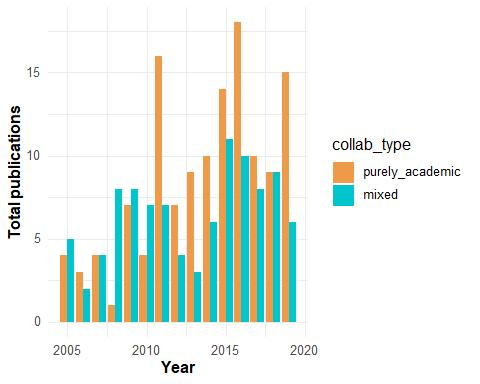
\includegraphics{orv_sys_rev_data_analysis_files/figure-latex/unnamed-chunk-14-1.jpeg}

\hypertarget{interventions}{%
\subsection{Interventions}\label{interventions}}

\hypertarget{types-of-interventions}{%
\subsubsection{Types of interventions}\label{types-of-interventions}}

\begin{longtable}[]{@{}llllr@{}}
\caption{Number of studies per intervention categories}\tabularnewline
\toprule
collab\_type & no\_vax & vax\_alongside & vax\_single & Total \\
\midrule
\endfirsthead
\toprule
collab\_type & no\_vax & vax\_alongside & vax\_single & Total \\
\midrule
\endhead
purely\_academic & 51.9\% (68) & 37.4\% (49) & 10.7\% (14) & 131 \\
mixed & 42.9\% (42) & 43.9\% (43) & 13.3\% (13) & 98 \\
Total & 48.0\% (110) & 40.2\% (92) & 11.8\% (27) & 229 \\
\bottomrule
\end{longtable}

\hypertarget{impact-of-vaccination}{%
\subsubsection{Impact of vaccination}\label{impact-of-vaccination}}

\begin{longtable}[]{@{}llllr@{}}
\caption{Conclusions about impact of vaccination}\tabularnewline
\toprule
collab\_type & yes & no & inconclusive & Total \\
\midrule
\endfirsthead
\toprule
collab\_type & yes & no & inconclusive & Total \\
\midrule
\endhead
mixed & 53.8\% (7) & 38.5\% (5) & 7.7\% (1) & 13 \\
purely\_academic & 42.9\% (6) & 35.7\% (5) & 21.4\% (3) & 14 \\
Total & 48.1\% (13) & 37.0\% (10) & 14.8\% (4) & 27 \\
\bottomrule
\end{longtable}

\begin{longtable}[]{@{}ll@{}}
\caption{Number of studies per disease for which vaccination was not
modelled}\tabularnewline
\toprule
disease & num\_of\_studies \\
\midrule
\endfirsthead
\toprule
disease & num\_of\_studies \\
\midrule
\endhead
influenza & 60.2\% (68) \\
ebola & 23.0\% (26) \\
dengue & 6.2\% (7) \\
tuberculosis & 3.5\% (4) \\
measles & 1.8\% (2) \\
cholera & 0.9\% (1) \\
malaria & 0.9\% (1) \\
mumps & 0.9\% (1) \\
pneumococcal\_disease & 0.9\% (1) \\
typhoid & 0.9\% (1) \\
varicella & 0.9\% (1) \\
Total & 100.0\% (113) \\
\bottomrule
\end{longtable}

\begin{longtable}[]{@{}llllr@{}}
\caption{Conclusions about impact of vaccination per
disease}\tabularnewline
\toprule
disease & yes & no & inconclusive & Total \\
\midrule
\endfirsthead
\toprule
disease & yes & no & inconclusive & Total \\
\midrule
\endhead
influenza & 42.9\% (9) & 42.9\% (9) & 14.3\% (3) & 21 \\
cholera & 100.0\% (3) & 0.0\% (0) & 0.0\% (0) & 3 \\
ebola & 0.0\% (0) & 0.0\% (0) & 100.0\% (1) & 1 \\
meningococcal\_meningitis & 0.0\% (0) & 100.0\% (1) & 0.0\% (0) & 1 \\
varicella & 100.0\% (1) & 0.0\% (0) & 0.0\% (0) & 1 \\
Total & 48.1\% (13) & 37.0\% (10) & 14.8\% (4) & 27 \\
\bottomrule
\end{longtable}

\hypertarget{secondary-objectives-of-review}{%
\section{Secondary objectives of
review}\label{secondary-objectives-of-review}}

\hypertarget{modelling-objectives}{%
\subsection{Modelling objectives}\label{modelling-objectives}}

\begin{longtable}[]{@{}llllr@{}}
\caption{Study objectives by collaboration type}\tabularnewline
\toprule
collab\_type & both & future & past & Total \\
\midrule
\endfirsthead
\toprule
collab\_type & both & future & past & Total \\
\midrule
\endhead
purely\_academic & 3.1\% (4) & 75.6\% (99) & 21.4\% (28) & 131 \\
mixed & 1.0\% (1) & 69.4\% (68) & 29.6\% (29) & 98 \\
Total & 2.2\% (5) & 72.9\% (167) & 24.9\% (57) & 229 \\
\bottomrule
\end{longtable}

\hypertarget{outbreak-types}{%
\subsection{Outbreak types}\label{outbreak-types}}

\begin{longtable}[]{@{}lllr@{}}
\caption{outbreak types by collaboration type}\tabularnewline
\toprule
collab\_type & hypothetical\_outbreak & real\_outbreak & Total \\
\midrule
\endfirsthead
\toprule
collab\_type & hypothetical\_outbreak & real\_outbreak & Total \\
\midrule
\endhead
purely\_academic & 52.7\% (69) & 47.3\% (62) & 131 \\
mixed & 45.9\% (45) & 54.1\% (53) & 98 \\
Total & 49.8\% (114) & 50.2\% (115) & 229 \\
\bottomrule
\end{longtable}

\hypertarget{modelling-objectives-and-outbreak-type-by-collaboration-types}{%
\subsection{Modelling objectives and outbreak type by collaboration
types}\label{modelling-objectives-and-outbreak-type-by-collaboration-types}}

\begin{longtable}[]{@{}ll@{}}
\caption{Number of studies per objective types}\tabularnewline
\toprule
objectives & num\_of\_studies \\
\midrule
\endfirsthead
\toprule
objectives & num\_of\_studies \\
\midrule
\endhead
future & 72.9\% (167) \\
past & 24.9\% (57) \\
both & 2.2\% (5) \\
Total & 100.0\% (229) \\
\bottomrule
\end{longtable}

\begin{longtable}[]{@{}llllr@{}}
\caption{Number of studies per objective by collaboration
type}\tabularnewline
\toprule
collab\_type & future & past & both & Total \\
\midrule
\endfirsthead
\toprule
collab\_type & future & past & both & Total \\
\midrule
\endhead
purely\_academic & 75.6\% (99) & 21.4\% (28) & 3.1\% (4) & 131 \\
mixed & 69.4\% (68) & 29.6\% (29) & 1.0\% (1) & 98 \\
Total & 72.9\% (167) & 24.9\% (57) & 2.2\% (5) & 229 \\
\bottomrule
\end{longtable}

\hypertarget{model-characteristics}{%
\subsection{Model characteristics}\label{model-characteristics}}

\hypertarget{individual-heterogeneity-agent-based-versus-compartmental-models}{%
\subsubsection{Individual heterogeneity: agent-based versus
compartmental
models}\label{individual-heterogeneity-agent-based-versus-compartmental-models}}

\begin{longtable}[]{@{}llllr@{}}
\toprule
collab\_type & compartments & agents &
individuals\_representation\_other & Total \\
\midrule
\endhead
purely\_academic & 80.9\% (106) & 18.3\% (24) & 0.8\% (1) & 131 \\
mixed & 76.5\% (75) & 21.4\% (21) & 2.0\% (2) & 98 \\
Total & 79.0\% (181) & 19.7\% (45) & 1.3\% (3) & 229 \\
\bottomrule
\end{longtable}

\hypertarget{spatial-heterogeneity}{%
\subsubsection{Spatial heterogeneity}\label{spatial-heterogeneity}}

\begin{longtable}[]{@{}lllr@{}}
\caption{Number of studies using models with explicit spatial
representation}\tabularnewline
\toprule
collab\_type & no & yes & Total \\
\midrule
\endfirsthead
\toprule
collab\_type & no & yes & Total \\
\midrule
\endhead
purely\_academic & 74.0\% (97) & 26.0\% (34) & 131 \\
mixed & 67.3\% (66) & 32.7\% (32) & 98 \\
Total & 71.2\% (163) & 28.8\% (66) & 229 \\
\bottomrule
\end{longtable}

\hypertarget{model-dynamics-deterministic-vs-stochastic}{%
\subsubsection{Model dynamics: deterministic vs
stochastic}\label{model-dynamics-deterministic-vs-stochastic}}

\begin{longtable}[]{@{}llllr@{}}
\caption{Model dynamics (deterministic versus
stochastic)}\tabularnewline
\toprule
collab\_type & both & deterministic & stochastic & Total \\
\midrule
\endfirsthead
\toprule
collab\_type & both & deterministic & stochastic & Total \\
\midrule
\endhead
purely\_academic & 5.3\% (7) & 71.8\% (94) & 22.9\% (30) & 131 \\
mixed & 7.1\% (7) & 53.1\% (52) & 39.8\% (39) & 98 \\
Total & 6.1\% (14) & 63.8\% (146) & 30.1\% (69) & 229 \\
\bottomrule
\end{longtable}

\hypertarget{modelling-methods}{%
\subsection{Modelling methods}\label{modelling-methods}}

\hypertarget{outcomes-measured}{%
\subsubsection{Outcomes measured}\label{outcomes-measured}}

\begin{longtable}[]{@{}ll@{}}
\caption{Number of studies per outcome measured}\tabularnewline
\toprule
outcome\_measured & n \\
\midrule
\endfirsthead
\toprule
outcome\_measured & n \\
\midrule
\endhead
final\_epidemic\_size & 24.8\% (86) \\
attack\_rate & 16.7\% (58) \\
timing\_of\_peak & 10.4\% (36) \\
cases\_averted & 10.1\% (35) \\
outbreak\_duration\_and\_timing & 8.1\% (28) \\
cost & 6.6\% (23) \\
intervention\_coverage & 4.0\% (14) \\
hospitalizations & 3.7\% (13) \\
case\_fatality & 2.9\% (10) \\
cumulative incidence & 2.9\% (10) \\
incidence & 2.9\% (10) \\
peak magnitude & 2.3\% (8) \\
r0 & 1.7\% (6) \\
peak size & 1.4\% (5) \\
total deaths & 1.4\% (5) \\
Total & 100.0\% (347) \\
\bottomrule
\end{longtable}

\includegraphics{orv_sys_rev_data_analysis_files/figure-latex/unnamed-chunk-29-1.jpeg}

\hypertarget{parametrization-methods}{%
\subsubsection{Parametrization methods}\label{parametrization-methods}}

\begin{longtable}[]{@{}
  >{\raggedright\arraybackslash}p{(\columnwidth - 16\tabcolsep) * \real{0.09}}
  >{\raggedright\arraybackslash}p{(\columnwidth - 16\tabcolsep) * \real{0.17}}
  >{\raggedright\arraybackslash}p{(\columnwidth - 16\tabcolsep) * \real{0.12}}
  >{\raggedright\arraybackslash}p{(\columnwidth - 16\tabcolsep) * \real{0.06}}
  >{\raggedright\arraybackslash}p{(\columnwidth - 16\tabcolsep) * \real{0.08}}
  >{\raggedright\arraybackslash}p{(\columnwidth - 16\tabcolsep) * \real{0.23}}
  >{\raggedright\arraybackslash}p{(\columnwidth - 16\tabcolsep) * \real{0.06}}
  >{\raggedright\arraybackslash}p{(\columnwidth - 16\tabcolsep) * \real{0.15}}
  >{\raggedleft\arraybackslash}p{(\columnwidth - 16\tabcolsep) * \real{0.03}}@{}}
\caption{How model parameters are obtained}\tabularnewline
\toprule
\begin{minipage}[b]{\linewidth}\raggedright
collab\_type
\end{minipage} & \begin{minipage}[b]{\linewidth}\raggedright
literature and expert\_opinion
\end{minipage} & \begin{minipage}[b]{\linewidth}\raggedright
literature and fitted
\end{minipage} & \begin{minipage}[b]{\linewidth}\raggedright
literature
\end{minipage} & \begin{minipage}[b]{\linewidth}\raggedright
expert\_opinion
\end{minipage} & \begin{minipage}[b]{\linewidth}\raggedright
literature and expert\_opinion and fitted
\end{minipage} & \begin{minipage}[b]{\linewidth}\raggedright
fitted
\end{minipage} & \begin{minipage}[b]{\linewidth}\raggedright
expert\_opinion and fitted
\end{minipage} & \begin{minipage}[b]{\linewidth}\raggedleft
Total
\end{minipage} \\
\midrule
\endfirsthead
\toprule
\begin{minipage}[b]{\linewidth}\raggedright
collab\_type
\end{minipage} & \begin{minipage}[b]{\linewidth}\raggedright
literature and expert\_opinion
\end{minipage} & \begin{minipage}[b]{\linewidth}\raggedright
literature and fitted
\end{minipage} & \begin{minipage}[b]{\linewidth}\raggedright
literature
\end{minipage} & \begin{minipage}[b]{\linewidth}\raggedright
expert\_opinion
\end{minipage} & \begin{minipage}[b]{\linewidth}\raggedright
literature and expert\_opinion and fitted
\end{minipage} & \begin{minipage}[b]{\linewidth}\raggedright
fitted
\end{minipage} & \begin{minipage}[b]{\linewidth}\raggedright
expert\_opinion and fitted
\end{minipage} & \begin{minipage}[b]{\linewidth}\raggedleft
Total
\end{minipage} \\
\midrule
\endhead
purely\_academic & 26.7\% (35) & 21.4\% (28) & 18.3\% (24) & 14.5\% (19)
& 9.9\% (13) & 6.9\% (9) & 2.3\% (3) & 131 \\
mixed & 24.5\% (24) & 28.6\% (28) & 14.3\% (14) & 7.1\% (7) & 19.4\%
(19) & 5.1\% (5) & 1.0\% (1) & 98 \\
Total & 25.8\% (59) & 24.5\% (56) & 16.6\% (38) & 11.4\% (26) & 14.0\%
(32) & 6.1\% (14) & 1.7\% (4) & 229 \\
\bottomrule
\end{longtable}

\hypertarget{validation-methods}{%
\subsubsection{Validation methods}\label{validation-methods}}

\begin{longtable}[]{@{}lllllr@{}}
\caption{How the model's performance is assessed}\tabularnewline
\toprule
collab\_type & none & data & another\_model & data\_and\_another\_model
& Total \\
\midrule
\endfirsthead
\toprule
collab\_type & none & data & another\_model & data\_and\_another\_model
& Total \\
\midrule
\endhead
purely\_academic & 71.8\% (94) & 27.5\% (36) & 0.8\% (1) & 0.0\% (0) &
131 \\
mixed & 53.1\% (52) & 42.9\% (42) & 3.1\% (3) & 1.0\% (1) & 98 \\
Total & 63.8\% (146) & 34.1\% (78) & 1.7\% (4) & 0.4\% (1) & 229 \\
\bottomrule
\end{longtable}

\hypertarget{sensitivity-analysis}{%
\subsubsection{Sensitivity analysis}\label{sensitivity-analysis}}

\begin{longtable}[]{@{}lllr@{}}
\toprule
model\_structure & no & yes & Total \\
\midrule
\endhead
deterministic & 58.2\% (85) & 41.8\% (61) & 146 \\
stochastic & 49.3\% (34) & 50.7\% (35) & 69 \\
both & 35.7\% (5) & 64.3\% (9) & 14 \\
Total & 54.1\% (124) & 45.9\% (105) & 229 \\
\bottomrule
\end{longtable}

\begin{longtable}[]{@{}lllr@{}}
\toprule
collab\_type & no & yes & Total \\
\midrule
\endhead
purely\_academic & 58.8\% (77) & 41.2\% (54) & 131 \\
mixed & 48.0\% (47) & 52.0\% (51) & 98 \\
Total & 54.1\% (124) & 45.9\% (105) & 229 \\
\bottomrule
\end{longtable}

\hypertarget{data-use-and-data-availability}{%
\subsubsection{Data use and data
availability}\label{data-use-and-data-availability}}

\begin{longtable}[]{@{}lllr@{}}
\caption{How often is the data used available for public
access}\tabularnewline
\toprule
collab\_type & yes & no & Total \\
\midrule
\endfirsthead
\toprule
collab\_type & yes & no & Total \\
\midrule
\endhead
purely\_academic & 82.5\% (52) & 17.5\% (11) & 63 \\
mixed & 58.7\% (37) & 41.3\% (26) & 63 \\
Total & 70.6\% (89) & 29.4\% (37) & 126 \\
\bottomrule
\end{longtable}

\hypertarget{code-availability}{%
\subsubsection{Code availability}\label{code-availability}}

\begin{longtable}[]{@{}lllr@{}}
\toprule
collab\_type & no & yes & Total \\
\midrule
\endhead
purely\_academic & 98.5\% (129) & 1.5\% (2) & 131 \\
mixed & 98.0\% (96) & 2.0\% (2) & 98 \\
Total & 98.3\% (225) & 1.7\% (4) & 229 \\
\bottomrule
\end{longtable}

\end{document}
